\documentclass[twoside]{article}
\usepackage{lmodern}
\usepackage{amssymb,amsmath}
\usepackage{ifxetex,ifluatex}
\usepackage{fixltx2e} % provides \textsubscript
\ifnum 0\ifxetex 1\fi\ifluatex 1\fi=0 % if pdftex
  \usepackage[T1]{fontenc}
  \usepackage[utf8]{inputenc}
\else % if luatex or xelatex
  \ifxetex
    \usepackage{mathspec}
  \else
    \usepackage{fontspec}
  \fi
  \defaultfontfeatures{Ligatures=TeX,Scale=MatchLowercase}
  \newcommand{\euro}{€}
\fi
% use upquote if available, for straight quotes in verbatim environments
\IfFileExists{upquote.sty}{\usepackage{upquote}}{}
% use microtype if available
\IfFileExists{microtype.sty}{%
\usepackage{microtype}
\UseMicrotypeSet[protrusion]{basicmath} % disable protrusion for tt fonts
}{}
\usepackage[margin=1in]{geometry}
\usepackage{hyperref}
\PassOptionsToPackage{usenames,dvipsnames}{color} % color is loaded by hyperref
\hypersetup{unicode=true,
            pdftitle={Reducing Corruption through Legislative Action A study of the Indian},
            pdfauthor={Devvart Poddar},
            pdfborder={0 0 0},
            breaklinks=true}
\urlstyle{same}  % don't use monospace font for urls
\usepackage{natbib}
\bibliographystyle{plainnat}
\usepackage{graphicx,grffile}
\makeatletter
\def\maxwidth{\ifdim\Gin@nat@width>\linewidth\linewidth\else\Gin@nat@width\fi}
\def\maxheight{\ifdim\Gin@nat@height>\textheight\textheight\else\Gin@nat@height\fi}
\makeatother
% Scale images if necessary, so that they will not overflow the page
% margins by default, and it is still possible to overwrite the defaults
% using explicit options in \includegraphics[width, height, ...]{}
\setkeys{Gin}{width=\maxwidth,height=\maxheight,keepaspectratio}
\setlength{\parindent}{0pt}
\setlength{\parskip}{6pt plus 2pt minus 1pt}
\setlength{\emergencystretch}{3em}  % prevent overfull lines
\providecommand{\tightlist}{%
  \setlength{\itemsep}{0pt}\setlength{\parskip}{0pt}}
\setcounter{secnumdepth}{5}

%%% Use protect on footnotes to avoid problems with footnotes in titles
\let\rmarkdownfootnote\footnote%
\def\footnote{\protect\rmarkdownfootnote}

%%% Change title format to be more compact
\usepackage{titling}

% Create subtitle command for use in maketitle
\newcommand{\subtitle}[1]{
  \posttitle{
    \begin{center}\large#1\end{center}
    }
}

\setlength{\droptitle}{-2em}
  \title{Reducing Corruption through Legislative Action\\
\LARGE A study of the Indian \textsl{Janlokpal Bill (2013)}}
  \pretitle{\vspace{\droptitle}\centering\huge}
  \posttitle{\par}
  \author{Devvart Poddar}
  \preauthor{\centering\large\emph}
  \postauthor{\par}
  \predate{\centering\large\emph}
  \postdate{\par}
  \date{December 16, 2016}


% Redefines (sub)paragraphs to behave more like sections
\ifx\paragraph\undefined\else
\let\oldparagraph\paragraph
\renewcommand{\paragraph}[1]{\oldparagraph{#1}\mbox{}}
\fi
\ifx\subparagraph\undefined\else
\let\oldsubparagraph\subparagraph
\renewcommand{\subparagraph}[1]{\oldsubparagraph{#1}\mbox{}}
\fi

\hypersetup{colorlinks=true, citecolor=blue, linkcolor=black}
\usepackage{setspace}
\usepackage{fancyhdr}
\pagestyle{fancy}
\fancyhead[OL,ER]{\large Legislaive Impact on Corruption}
\fancyhead[EL,OR]{\thepage}
\fancyfoot[L]{\small Devvart Poddar}
\fancyfoot[R]{\small Hertie School of Governance}
\fancyfoot[C]{}

\begin{document}
\maketitle

{
\setcounter{tocdepth}{2}
\tableofcontents
}
\pagebreak

\section{Introduction}\label{introduction}

Corruption has become a major flash point in the Indian political debate
post multiple scandals which rocked India in 2011. A major policy issue
at the height of the debate was the creation of an independent
corruption watchdog through legislative assent; the \emph{Jan Lokpal
Act} of 2013. The watchdog itself was recommended as far back as 1969,
but was never created in the fluid political scenario.

There have been several studies which have looked at the impact of
legislative actions in reducing corruption
\citep[See][\citet{prado2016brazilian}]{quah2007combating}, however the
results of the reforms are mixed. While Singapore was successful in the
enforcement of their reforms in the city-state, similar changes in
Brazil failed to reduce corruption. Moreover the study of corruption, be
definition, is difficult to measure. Corruption is undertaken in the
shadows of economic and political actions, and is notoriously difficult
to predict. Watchdogs like the Transparency International (TI) use
perception surveys which are conducted wig \emph{experts} around the
work. Other NGOs in India like the Center for Media Studies (CMS) also
measure corruption through surveys, albeit with citizens across the
country.

However, there are several issues which plague expert surveys. They are
a subjective measure of perception which may be impacted by Individual
biases. As the same individual is not studied across her lifetime, it is
hard to dis aggregate the idiosyncratic biases from actual corruption.
Thus I turn to the use of Indian media data sets to create an unbiased
indicator of corruption.

\section{Methodolgy}\label{methodolgy}

\subsection{Media as Data}\label{media-as-data}

This study is not the first to use media as a source of data for
economic research. \citet{jansen2005talking} use media to identify the
impact of communications from the European Central Bank (ECB) on
exchange rate volatility. Similarly \citet{baker2015measuring} use media
data to identify and measure economic policy uncertainty in 15
countries. However to the best of the author's knowledge, no study has
used media as an indicator for corruption.

For the study, nearly 19000 articles were scrapped from
\href{\%22https://news.google.com/\%22}{Google News} for a period of 8
years; from 2008 \textasciitilde{} 2016. The frequency of the articles
is showcased in Figure 1 below. They identify two main changes in the
approach of the study; \emph{firstly} due to idiosyncrasies of Google
News, there is a jump in the number of articles on corruption for the
last month of the study. This is a clear outlive, possibly due to
sorting on the basis of the time of the scraping. Those months will be
ignored in the analysis.

\emph{Secondly} we see a clear time trend and a seasonal component to
the number of articles. While the time trend was expected, as the news
media has evolved rapidly to growing digitization, the seasonal trend
was not expected. Regardless moving forward, the study will take into
account the time trend and seasonality in all further analysis.

\begin{figure}[htbp]
\centering
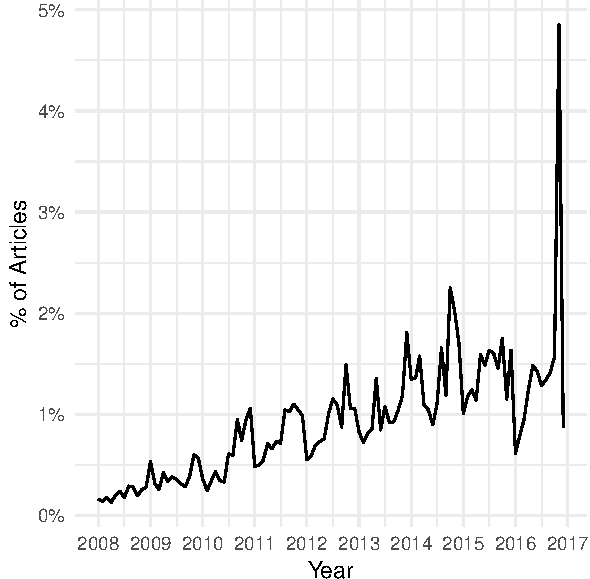
\includegraphics{FinalPaper_files/figure-latex/freqplot-1.pdf}
\caption{Trend in articles on corruption in India}
\end{figure}

\subsection{Insights from Text}\label{insights-from-text}

The media data sets are incredibly insightful in terms of the richness
of the data provided. We can measure corruption up-till the states, and
even cities to a certain extent. The wealth of data also allows analysis
of the different aspects of corruption itself, i.e.~the forms of
corruption. We can also track the growth in corruption by different
groups (corporate houses, politicians, NGOs etc) separately. However
those are beyond the scope of this research. For the study, we will
create a indicator of corruption using text, for the different states in
India.

\subsubsection{Lemmatisation and Natural Language
Programming}\label{lemmatisation-and-natural-language-programming}

The first stage of the analysis involves the use of \textbf{Treetagger},
a tool developed by \citet{schmid1994treetagger} for annotating text
with part-of-speech tags. \textbf{Treetagger} can annotate over 13
languages, and provides us with the \emph{lemma}, the root form of a
word. Lemmatisation is a powerful method of reducing the complexity of
text, particularly in form of the different tenses, without changing the
meaning of the text. The lemmatisation is further restricted on
adjectives and adverbs, i.e.~any word that qualifies / describes the
context of the article is not modified. This would help in the
succeeding stages to help create an index of corruption.

The text is also cleaned using a Natural Language Programming (NLP)
framework \citep[See][ for a definative guide to
NLP]{manning1999foundations}. Natral Language Programming in an
intersection of comupational-linuistics and artificial intelligence,
aiming to make text \emph{machine-readable}. As such, it is the base of
all systems that depend upon understanding and analysing text (Siri from
Apple is one of the best examples. The core component of Siri,
understanding the \emph{human} command, works through applications of
NLP. See \citet{Dworetzky}).

For the study, NLP is used primarly to detect \emph{negation} and
\emph{emphasis}. Thus words like \emph{not} and \emph{no} which invert
the meaning of a sentence are taken into account when building the
index, as well as emphasis words like \emph{very} and \emph{greatly}
which increase the emphasis of the sentence. Moreover the indicator is
built at a sentence level, i.e we do not look at the entire text, but a
window of words around corruption. This allows the index to identify the
rising and falling trends of corruption in the different states.

To better understand the techniques of lemmatisation, and how it helps
in creating the index, a small example is given below. The following
quote is taken from a article on corruption against a prominent Indian
politician;

\begin{quote}
\emph{One of India's most colourful and controversial politicians,
Jayaram Jayalalitha, has been sentenced to jail for four years on
corruption charges in a case that has lasted for 18 years. The chief
minister of the southern state of Tamil Nadu was found guilty of
amassing wealth of more than \$10m (£6.1m) which was unaccounted for.
She has to pay a 1bn rupee (\$16m; £10m) fine and resign as chief
minister.} (\citet{bbc2014})
\end{quote}

Upon cleaning and lemmatising, the text will change to as below;

\begin{quote}
\emph{one indias colourful controversial politician jayaram jayalalitha
sentence jail four year corruption charge case last year chief minister
southern state Tamil nadu find guilty amass wealth unaccounted pay bn
rupee fine resign chief minister}
\end{quote}

\subsubsection{States and corruption}\label{states-and-corruption}

\subsection{Regression Framework}\label{regression-framework}

\section{Results}\label{results}

\section{Conclusions}\label{conclusions}

\renewcommand\refname{References}
\bibliography{Bibtex.bib}

\end{document}
